\linespread{1.5}
Um exemplo clássico da ocorrencia de equações diferenciais de segunda ordem é o modelo do fluxo de corrente elétrica no circuito RLC, representado na figura abaixo.
\begin{figure}[H]
    \centering
    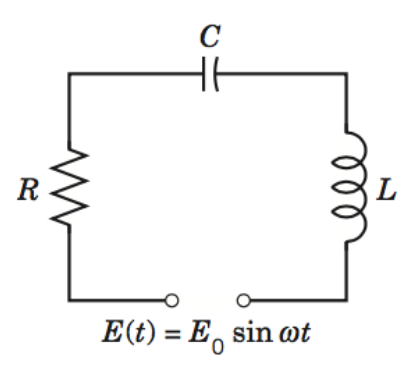
\includegraphics[width=0.5\linewidth]{fig/edo32}
\end{figure}

O fluxo de corrente elétrica, \textit{I(t)}, no circuito em série RLC, medido em Ampère (\textit{A}), é uma função do tempo, t, e pode ser escrito como:
\begin{equation}
    \label{eq:edo321}
    I(t) = \frac{dQ(t)}{dt},
\end{equation}

sendo Q(t) a carga elétrica total, medida em Coulomb (\textit{C}). A resistência, em Ohm ($\Omega$), a capacitância, em Farad (\textit{F}), e a indutância \textit{L}, em Henry (\textit{H}), são constantes positivas que supomos ser conhecidas no problema. A tensão (\textit{U}), em Volt (\textit{V)}), é uma função do tempo. O fluxo de corrente no circuito é governado pela segunda lei de Kirchhoff.  Assim, a equação diferencial de segunda ordem que descreve o comportamento da corrente elétrica em função do tempo nesse circuito resulta da aplicação das seguintes leis:
\begin{enumerate}
    \item Lei de Kirchhoff: Em um circuito fechado, a tensão aplicada é igual à soma das quedas de tensão no resto do circuito.
    \item Lei de Ohm: A diferença de potencial aplicada (\textit{U}) aos terminais de um resistor metálico, mantido à temperatura constante, é diretamente proporcional à intensidade de corrente elétrica que o atravessa. Matematicamente:
    \begin{equation}
        U=RI
        \label{eq:edo322}
    \end{equation}
    \item A queda de tensão, \textit{U}, através de um indutor, \textit{L}, é proporcional à taxa de variação da corrente elétrica, \textit{I}. Isto é:
    \begin{equation}
        U = L\frac{dI}{dt}
        \label{eq:edo323}
    \end{equation}
    \item A queda de tensão, \textit{U}, através de um capacitor, \textit{C}, é proporcional ao valor da carga elétrica, \textit{Q}, armazenada no condutor, ou seja,
    \begin{equation}
        \label{eq:edo324}
        U = QC
    \end{equation}
\end{enumerate}
Portanto, pela lei de Kirchhoff, temos:
\begin{equation}
    L\frac{dI(t)}{dt} + RI(t) + \frac{1}{C}Q(t) = U(t)    \label{eq:edo325}
\end{equation}

Derivando-se a equação (\ref{eq:edo325}) em relação a \textit{t}, obtemos:
\begin{equation}
    L\frac{d^2I(t)}{dt^2} + R\frac{dI(t)}{dt} + \frac{1}{C}I(t) = \frac{dU(t)}{dt}
    \label{eq:edo326}
\end{equation}
Considerando $E(t) = E_0sin(wt)$, na equação (\ref{eq:edo326}), determine:
\begin{itemize}
    \item[\textbf{a)}] Ache a solução geral da equação diferencial de 2ª ordem da equação (\ref{eq:edo326});
    \item[\textbf{b)}] Determine a carga total, $Q(t)$, a partir da solução obtida no item \textbf{a)};
    \item[\textbf{c)}] Determine a corrente $I(t)$ em um circuito RLC (Figura acima), sendo $R = 11\Omega$, $L = 0.1H$, $C = 10^{-2}F$, o qual está conectado a uma fonte $U(t) = 110sin(60.2\pi t) = 110sin(377t)$. Assuma que a corrente e a carga do capacitor são 0 quando $t=0$.
\end{itemize}
